% !TeX program = xelatex
\documentclass{report}

\PassOptionsToPackage{intoc}{nomencl}

%───────── Plantilla, portadas y contraportada ─────────────────────────
\usepackage{template/sty_files/template-TFGenglish-uma}

\usepackage{template/sty_files/cotutor_cover-blueuma}
\usepackage{template/sty_files/cotutor_cover-whiteuma}

\usepackage{template/sty_files/plain_cover-blueuma}
\usepackage{template/sty_files/plain_cover-whiteuma}

\usepackage{template/sty_files/backcover-uma}

%───────── Paquetes auxiliares ─────────────────────────────────────────
\usepackage{blindtext}
\usepackage{amssymb}       % \mathbb, \mathcal...
\usepackage{mwe}               % imágenes de prueba
\usepackage{csquotes}
\usepackage[
  backend=biber,
  style=numeric,
  sorting=nyt,
  maxbibnames=10,
  giveninits=true
]{biblatex}
\addbibresource{references.bib}

\graphicspath{{figures/}}

%======================================================================
\begin{document}

\frontmatter
%────────────────────── Blue front cover ───────────────────────────────
\MakeBlueUMACover{
  degree     = {Grado en Ingeniería Informática},
  mencion    = {Ingeniería del Software},
  titleES    = {Detección de anomalías en robots industriales y activos móviles (AGV/AMR) mediante Machine 
Learning para Mantenimiento Predictivo. },
  titleEN    = {Anomaly Detection in Industrial Mobile Assets (AGV/AMR) using Machine Learning for Predictive 
Maintenance },
  author     = {Rafael Sáez Arana},
  tutor      = {Cristian Martin Fernández},
  cotutor    = {Bartolomé Rubio Muñoz},
  dept       = {Departamento de Lenguajes y Ciencias de la Computación},
  cityDate   = {Málaga, \today},
  logoLeft   = {template/logos/NEG-uma-logo.png},
  logoRight  = {template/logos/NEG-etsi-logo.png}
}

%────────────────────── White front cover ──────────────────────────────
\MakeWhiteUMACover{
  degree      = {Grado en Ingeniería Informática},
  mencion     = {Ingeniería del Software},
  titleES     = {Detección de anomalías en robots industriales y activos móviles (AGV/AMR) mediante Machine 
Learning para Mantenimiento Predictivo. },
  titleEN     = {Anomaly Detection in Industrial Mobile Assets (AGV/AMR) using Machine Learning for Predictive 
Maintenance },
  author      = {Rafael Sáez Arana},
  tutor       = {Cristian Martin Fernández},
  cotutor     = {Bartolomé Rubio Muñoz},
  dept        = {Departamento de Lenguajes y Ciencias de la Computación},
  cityDate    = {MÁLAGA, \today},
  defenseDate = {septiembre de 2025},
  logoLeft    = {template/logos/POS-uma-logo.png},
  logoRight   = {template/logos/POS-etsi-logo.png}
}

%────────────────────── Resumen / Abstract ─────────────────────────────
% !TeX root = ../main.tex
\renewcommand{\abstractname}{Resumen}
\begin{abstract}
En el marco de la transición hacia la Industria 4.0, los activos industriales y vehículos de guiado autónomo han evolucionado hacia sistemas capaces de emitir volúmenes continuos de telemetría en tiempo real, generando un gran caudal de información. Sin embargo, la simple recolección de estos datos no aporta valor operativo por sí sola. Únicamente mediante un procesamiento y análisis adecuados es posible transformar dichos datos en conocimiento útil para la toma de decisiones estratégicas.
De ahí surge la idea de este proyecto, desarrollado en colaboración con EDAG, entidad de referencia en el sector industrial.\\ 

A pesar del avance en el mantenimiento predictivo durante los últimos años, existe una brecha notable entre los estudios teóricos sobre detección de anomalías y su aplicación efectiva en entornos de producción. Esta limitación se debe principalmente a la complejidad en la recolección de datos de calidad, al dinamismo de los entornos industriales y a la necesidad de procesar la información con bajas latencias para actuar antes de que ocurra una avería.\\

Para dar respuesta a esta problemática, este proyecto presenta una solución integral para la detección de anomalías en tiempo real sobre una flota de robots móviles. El sistema se compone de una infraestructura distribuida de ingesta y procesamiento continuo de datos, una capa de almacenamiento histórico optimizada para series temporales y un módulo analítico basado en aprendizaje automático para la identificación de comportamientos anómalos. Todo el conjunto se completa con una herramienta visual de monitorización y alertas para el personal de planta, desarrollada bajo una arquitectura limpia, desacoplada y escalable.

\medskip
\noindent\textbf{Palabras clave:} IIoT, Mantenimiento Predictivo, Detección de Anomalías, Aprendizaje Automático, Robots Móviles, Industria 4.0, Data Lakehouse, Arquitectura Medallón.
\end{abstract}
% !TeX root = ../main.tex
\renewcommand{\abstractname}{Abstract}
\begin{abstract}
As part of the transition towards Industry 4.0, industrial assets and autonomous guided vehicles have evolved into systems capable of transmitting continuous streams of real-time telemetry, generating a vast amount of information. However, simply collecting this data does not, in itself, provide any operational value. Only through appropriate processing and analysis is it possible to transform this data into useful knowledge for strategic decision-making.
This is where the idea for this project came from, developed in collaboration with EDAG, a leading organisation in the industrial sector.\\

Despite the progress made in predictive maintenance in recent years, there remains a significant gap between theoretical studies on anomaly detection and their effective application in production environments. This limitation is mainly due to the complexity of collecting high-quality data, the dynamic nature of industrial environments and the need to process information with low latency in order to take action before a failure occurs.\\

To address this issue, this project presents a comprehensive solution for real-time anomaly detection across a fleet of mobile robots. The system comprises a distributed infrastructure for continuous data ingestion and processing, a historical storage layer optimised for time series, and an analytics module based on machine learning for identifying anomalous behaviour. The system is rounded off by a visual monitoring and alerting tool for plant staff, developed using a clean, decoupled and scalable architecture.\\
\medskip
\noindent\textbf{Keywords:} IIoT, Predictive Maintenance, Anomaly Detection, Machine Learning, AGV, AMR, Industrial Robots, Industry 4.0, Data Lakehouse, Medallion Architecture.
\end{abstract}


%──────────────── Agradecimientos ──────────────────────────────────────
% Sección opcional, si no se quiere usar, borrar el entorno umaacknowledgments

% Descomentar si los vas a escribir en inglés
% \SetAcknowledgmentsName{Acknowledgments} 
\begin{umaacknowledgments}

\end{umaacknowledgments}

%────────────────────── Índice y listas ────────────────────────────────
\cleardoublepage
\tableofcontents
\cleardoublepage
\listoffigures
\cleardoublepage
\listoftables
\cleardoublepage

%────────────────────── Nomenclatura ───────────────────────────────────
% ── Nomenclature ──────────────────────────────────────────────────────
% Add new entries with: \nomenclature{acronym}{definition}
% ──────────────────────────────────────────────────────────────────────
\nomenclature{AGV}{Automated Guided Vehicle}
\nomenclature{AMR}{Autonomous Mobile Robot}
\nomenclature{AI}{Artificial Intelligence}
\nomenclature{ML}{Machine Learning}
\nomenclature{IoT}{Internet of Things}
\nomenclature{IIoT}{Industrial Internet of Things}
\nomenclature{VDA 5050}{Verband der Automobilindustrie 5050}
\nomenclature{GRU}{Gated Recurrent Unit}
\nomenclature{LSTM}{Long Short-Term Memory}
\nomenclature{GRU-AE}{Gated Recurrent Unit Autoencoder}
\nomenclature{LSTM-AE}{Long Short-Term Memory Autoencoder}
\nomenclature{RCA}{Root Cause Analysis}
\nomenclature{XAI}{Explainable Artificial Intelligence}
\printnomenclature
\cleardoublepage

\mainmatter
%────────────────────── Cuerpo ─────────────────────────────────────────
% https://en.wikipedia.org/wiki/Standing_on_the_shoulders_of_giants 
% !TeX root = ../main.tex
\chapter{Introduction}
\label{chap:introduction}

\section{Motivation}
Industry 4.0 is no longer just a concept, but a reality transforming factories worldwide. 
The arrival of these emerging technologies opens up vast opportunities to optimize production processe, shifting the focus from mere automation toward creating truly intelligent factories.\\

A key enabler of Industry 4.0 is the deployment of Automated Guided Vehicles (AGVs) and Autonomous Mobile Robots (AMRs), which are capable of navigating autonomously through factories, warehouses, and complex environments. \\

Their adoption across industries continues to surge, with market research pointing to sustained, strong growth in the coming years \cite{imarc2026agv}.\\

\begin{figure}[ht]
  \centering
  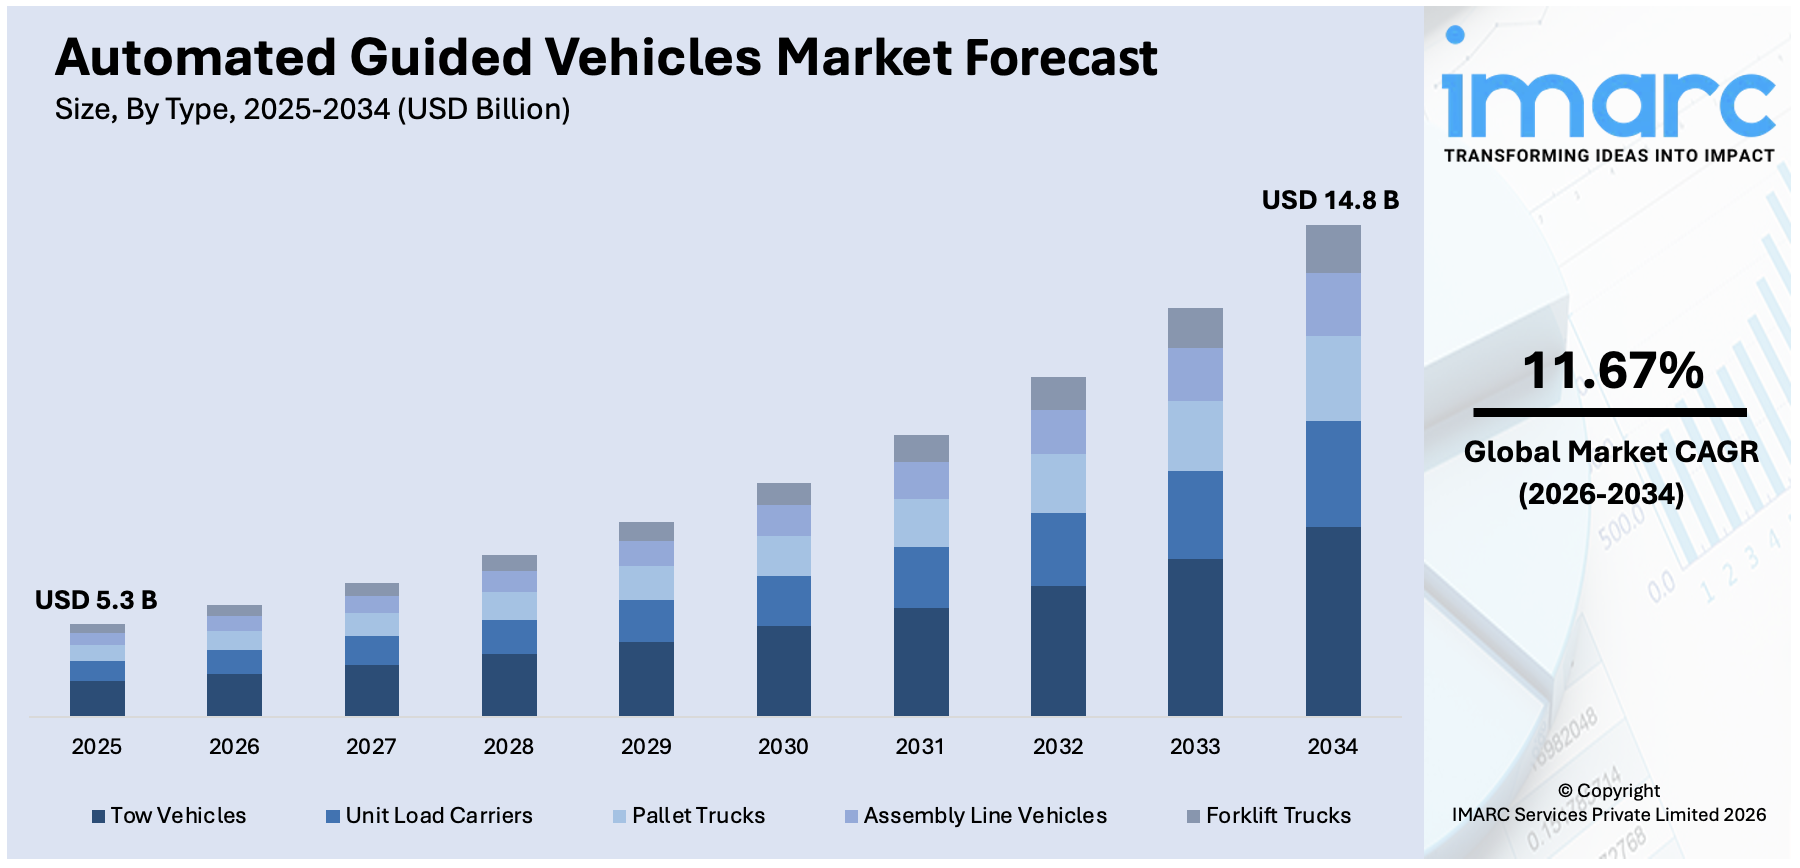
\includegraphics[width=.85\linewidth]{marquetForecastAgv.png}
  \caption{Global AGV market forecast (2025--2034). Source: IMARC Group~\cite{imarc2026agv}.}
  \label{fig:agv-market-forecast}
\end{figure}

Because these vehicles play a vital role in production, any failure can paralyze the assembly line, resulting in substantial financial losses. 
Studies reveal that unexpected downtime can range from \$36,000 per hour in fast-moving consumer goods to upwards of \$2.3 million per hour in the automotive sector \cite{siemens2024Cost}. 
Consequently, preventing such disruptions is not merely an operational challenge, but a critical financial priority for modern manufacturers.\\

A promising solution to this challenge is predictive maintenance, which can significantly reduce vehicle failures and the associated costs of unplanned downtime. 
The literature on machine learning for anomaly detection is extensive, however, a significant gap remains between theoretical studies and real-world implementation, as researchers encounter major hurdles when scaling proposed solutions to production environments \cite{paleyes2022challenges}.\\

Through a review of this literature, four key limitations emerge as critical factors when developing a real-time anomaly detection system for AGVs and AMRs \cite{benecki2024agv}:
\begin{itemize}
\label{item:challenges}
    \item \textbf{High-volume data management and processing:} Managing and automatically processing vast amounts of data, ensuring not only scale handling but also the quality and relevance of the ingested information.
    \item \textbf{Dynamism of industrial environments:} The inherently dynamic nature of manufacturing settings requires continuous adaptation to shifting conditions and novel anomaly types.
    \item \textbf{Ambiguity of anomalies:} The challenge of accurately classifying anomalies to establish a robust mapping between newly detected anomalies and known failure modes.
    \item \textbf{Real-time integration of machine learning models:} Deploying machine learning inference within real-time environments to enable immediate anomaly detection and automated response.
\end{itemize}

To complement the core challenges identified in the literature, an additional constraint must be considered in this work: the total lack of labeled historical error data, which precludes the use of supervised learning approaches.\\

\section{Objectives}
As demonstrated in the previous section, AGVs and AMRs are fully integrated into Industry 4.0 processes. While they drive automation across the production line, their critical role implies that any asset failure can lead to a complete halt in production. Furthermore, although numerous studies validate the effectiveness of machine learning for anomaly detection, translating these approaches into real-world production environments presents significant technical limitations.\\

To address these challenges, this project aims to design and implement a fully decoupled, end-to-end architecture for real-time anomaly detection. Broadly speaking, the proposed pipeline encompasses the entire data lifecycle: from simulated AGV telemetry generation, real-time data ingestion, processing, and persistence, to unsupervised machine learning anomaly detection and interactive visualization of diagnostic metrics.\\

To achieve this overarching goal, the project is structured into five specific technical objectives:
\begin{enumerate}
    \item \textbf{Adaptation of the VDA 5050\cite{vda5050standard} Simulator\cite{bostanciVda5050}:} 
    Due to hardware constraints and limited access to physical AGVs, utilizing real industrial data is often unfeasible. Therefore, a Rust-based VDA 5050 simulator is to be adapted to generate realistic telemetry streams. The simulation is extended beyond pure protocol compliance to model real-world robot physics and key health metrics, including motor current, motor voltage, motor temperature, linear velocity, and battery state. Generative AI tool(Claude Sonnet 3.5) is to be leveraged to assist in extending the Rust codebase.

    \item \textbf{Real-Time Data Pipeline Implementation:} 
    To process raw telemetry streams before they reach downstream machine learning components, Apache Spark is used to ingest raw streams, cleanse null fields, append ingestion timestamps, and standardize data structures. Cleaned events are to be published to a Redpanda event broker. This Kafka-compatible streaming layer decouples system modules, allowing independent producers and consumers to interact seamlessly.

    \item \textbf{Data Lakehouse and Medallion Architecture\cite{dey2026lakehouse}:} 
    To ensure scalable, long-term persistence, a Data Lakehouse paradigm is adopted. It combines the cost-effective storage of object repositories (S3-compatible bucket) with the structured, ACID-compliant query capabilities of Apache Iceberg. Data is to be organized following a Medallion Architecture:
    \begin{itemize}
        \item \textbf{Bronze Layer:} To store raw, unprocessed telemetry streams exactly as received.
        \item \textbf{Silver Layer:} To contain cleaned, validated, and enriched data with added ingestion metadata.
        \item \textbf{Gold Layer:} To hold business-level aggregations, detected anomalies, and analytical outputs.
    \end{itemize}

    \item \textbf{Deep Learning for Anomaly Detection:} 
    Serving as the core analytical engine, this component focuses on unsupervised anomaly detection using deep learning frameworks (PyTorch). Following a review of current methodologies, a deep learning model (e.g., Autoencoder) is to be deployed to detect subtle telemetry deviations. Furthermore, the objective extends beyond raw mathematical score calculation to map detected anomalies to clear, non-ambiguous diagnostic labels for human interpretability.

    \item \textbf{Visualization and Monitoring Layer:} 
    To present actionable insights to operational staff, telemetry and anomaly scores are to be persisted in QuestDB—a high-performance time-series database. Grafana dashboards then query QuestDB to display real-time metrics, system health status, and historical anomaly alerts.
\end{enumerate}

This multi-layered approach not only supports live monitoring, but through the Medallion Architecture and Iceberg time-travel capabilities, it allows historical raw data (Bronze layer) to be reprocessed whenever model architectures or machine learning requirements evolve.

\subsection{Industrial Context and Collaboration}
This project is carried out in collaboration with EDAG Engineering Group. 
As an international engineering service provider for the automotive and manufacturing industries, EDAG actively develops cutting-edge Industry 4.0 solutions. 
Developing this project during an internship at EDAG provides direct insight into real-world industrial environments, system requirements, and deployment constraints. 
Specifically, this work contributes to the \textbf{Metys} project \cite{edagMetys}, an initiative aimed at optimizing software development and smart production workflows.

\section{Scope and Limitations}
The scope of this project encompasses the end-to-end design and implementation of a real-time anomaly detection system for Autonomous Guided Vehicles (AGVs) and Autonomous Mobile Robots (AMRs). 

It is important to emphasize that this work does not focus on prescribing automated corrective actions or actively preventing anomalies; rather, it is restricted to their detection and operational visualization. Consequently, determining the appropriate mitigation strategies remains at the discretion of the end user or plant operator.

Furthermore, the operational scope of this project is subject to several specific constraints and limitations:

\begin{itemize}
    \item \textbf{Industrial Environment Constraints:} The development process was conducted in close collaboration with an industrial partner. While this provided access to real-world operational contexts and expert technical support, it also imposed fixed technical requirements. Specifically, non-functional constraints—such as adhering to the VDA 5050 protocol standard \cite{vda5050}—were mandatory to ensure seamless integration into the target industrial platform \cite{edagMetys}.
    
    \item \textbf{Dependency on Simulated Telemetry and Anomaly Data:} Due to the unavailability of physical robot fleets for continuous data acquisition, the Machine Learning models are trained exclusively on telemetry generated by simulated AGV/AMR fleets. Consequently, the model may struggle to fully generalize to the complex stochastic behavior inherent to physical production environments. Furthermore, because real failure logs were unavailable, performance evaluation is conducted using synthetically injected anomalies. While testing on a physical AMR platform remains a prospective goal, replicating complex mechanical and electrical anomalies on actual hardware carries significant economic and operational costs.
    
    \item \textbf{Context Sensitivity and False Positives:} Unsupervised Machine Learning models rely on establishing a nominal baseline from the assets' operational telemetry. Consequently, any valid operational state or contextual change omitted from the training dataset—such as an unseen payload weight being transported or an unfamiliar speed setting—will inevitably be misclassified as an anomaly during inference, resulting in false positives.
    
    \item \textbf{Computational Constraints:} System throughput and real-time processing capabilities are bounded by the hardware resources (CPU, RAM, and storage) of the local host machine used during development. As a result, this prototype does not fully capture the performance dynamics or dynamic scalability of a cloud cluster deployment.
    
    \item \textbf{Resource and Time Constraints:} Due to the fixed timeframe and individual nature of an academic thesis, the project scope was intentionally bounded to deliver a fully functional Proof of Concept (PoC). Consequently, exhaustive experimental exploration of complex MLOps pipelines and alternative model architectures was beyond the achievable scope.
\end{itemize}

\section{Document structure}
To be done\dots
% !TeX root = ../main.tex
\chapter{State of the Art}

\section{Taxonomy of Deep Anomaly Detection Paradigms}

To build a solid theoretical groundwork for real-time telemetry analytics in autonomous mobile robotics, this section examines the comprehensive taxonomy of deep anomaly detection formulated by Pang et al. \cite{pang2021deep}. As depicted in Figure~\ref{fig:anomaly-detection-taxonomy}, algorithmic approaches in deep learning are structured into three main modeling paradigms based on the formulation of feature representation learning and its coupling with the anomaly scoring objective \cite{pang2021deep}.

\begin{figure}[htbp]
  \centering
  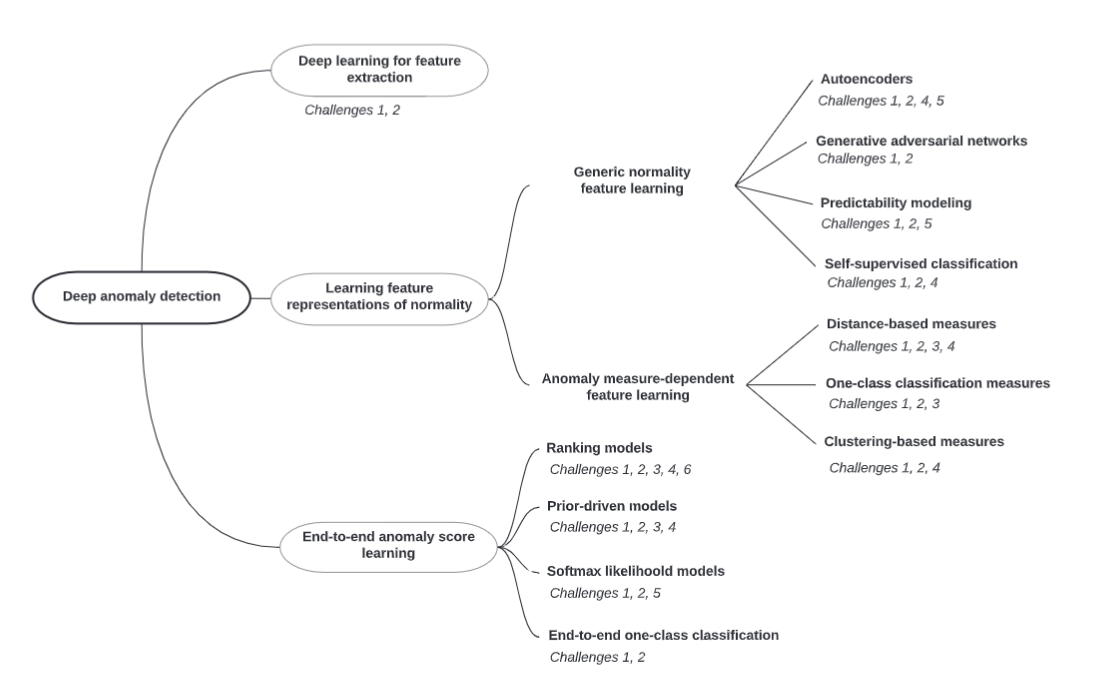
\includegraphics[width=0.90\linewidth]{anomalyDetectionTaxonomyACMComputingSurvey.png}
  \caption{Taxonomy of deep anomaly detection techniques categorized by feature representation learning and objective function formulation \cite{pang2021deep}.}
  \label{fig:anomaly-detection-taxonomy}
\end{figure}

\subsection{Categorization of Algorithmic Methodologies}

\begin{enumerate}
    \item \textbf{Deep Learning for Feature Extraction:} This two-stage framework employs a pre-trained deep neural network strictly as a static feature transformation layer, projecting high-dimensional raw inputs $\mathbf{x} \in \mathbb{R}^D$ into a lower-dimensional latent representation $\mathbf{z} \in \mathbb{R}^d$. Conventional shallow anomaly detectors, such as Isolation Forests ($i$Forest) or Local Outlier Factor (LOF), are subsequently applied to the extracted features. While computationally convenient, this decoupled methodology exhibits a major theoretical drawback: the feature extraction architecture is trained independently of the anomaly scoring criterion, potentially discarding subtle non-linear signals critical for fault detection \cite{pang2021deep}.
    
    \item \textbf{Learning Feature Representations of Normality:} Rather than relying on task-agnostic representations, this paradigm constructs custom feature spaces explicitly optimized to model the structural properties of nominal system operation \cite{pang2021deep}. Based on the underlying optimization objective, it is divided into two major sub-categories:
    \begin{itemize}
        \item \textit{Generic Normality Feature Learning:} This approach leverages self-supervised or generative surrogate tasks to learn latent data representations under nominal conditions \cite{pang2021deep}. Key examples include \textbf{Autoencoders (AE)} and \textbf{Generative Adversarial Networks (GANs)}. Autoencoders impose an information bottleneck that compresses input streams into a constrained latent space and subsequently reconstructs them. Observations yielding reconstruction residuals above a dynamic statistical threshold are flagged as anomalous \cite{pang2021deep, blazquez2021review}.
        \item \textit{Anomaly Measure-Dependent Feature Learning:} This framework optimizes feature representations directly within dedicated geometric or metric spaces \cite{pang2021deep}. A representative architecture is \textbf{Deep One-Class Classification (Deep SVDD)} \cite{ruff2018deep}, which trains a neural network to map nominal data points inside a minimal-volume hypersphere in feature space, penalizing observations mapped beyond this boundary \cite{ruff2018deep}.
    \end{itemize}
    
    \item \textbf{End-to-End Anomaly Score Learning:} This unified paradigm eliminates intermediate representation steps by directly training custom neural architectures to output continuous anomaly scores in an end-to-end backpropagation process, employing specialized ranking loss functions or prior-driven distribution matching metrics \cite{pang2021deep}.
\end{enumerate}

\subsection{Methodological Selection and Alignment with AGV Telemetry Constraints}

Evaluating this taxonomy against the operational requirements of AGV and AMR telemetry processing provides a clear rationale for algorithm selection in this project:

\begin{itemize}
    \item \textbf{Multivariate High-Dimensional Temporal Coupling:} Industrial telemetry emitted by mobile fleets comprises multiple synchronized time series (e.g., motor current, motor voltage, motor temperature, linear velocity, and battery state) exhibiting complex non-linear spatial-temporal correlations \cite{benecki2024agv, blazquez2021review}. \textit{Generic Normality Feature Learning}, specifically \textbf{Recurrent Autoencoder architectures (GRU-AE / LSTM-AE)}, excels at capturing these latent temporal dependencies while addressing high dimensionality and low anomaly recall rates \cite{pang2021deep, blazquez2021review}.
    
    \item \textbf{Low-Latency Ingestion in Medallion Architecture:} Deploying real-time anomaly detection within a time-series Data Lakehouse demands deterministic inference performance \cite{benecki2024agv, paleyes2022challenges}. Recurrent Autoencoders exhibit a linear computational complexity $\mathcal{O}(T)$ per time window, enabling low-latency execution in the continuous stream processing pipeline (Silver layer) before pushing structured alerts to the observation system.
    
    \item \textbf{Granular Root-Cause Explainability:} By decomposing the total reconstruction residual $\|\mathbf{X} - \hat{\mathbf{X}}\|^2$ along individual telemetry channels, generic reconstruction models provide explicit variable-level attribution, transforming abstract anomaly scores into interpretable diagnostic data for maintenance technicians \cite{pang2021deep}.
\end{itemize}

Consequently, this work adopts a \textbf{Gated Recurrent Unit Autoencoder (GRU-AE) with reconstruction residual decomposition} as the core analytical engine for real-time AGV fleet monitoring.

//Revisar
\section{Scalable Real-Time Telemetry Pipelines and Data Lakehouse Architecture}

Processing high-frequency telemetry streams generated by autonomous mobile fleets poses severe data engineering challenges regarding ingestion throughput, low-latency transformations, and transactional persistence \cite{mohna2024medallion}. Traditional data warehouse architectures struggle with the velocity and semi-structured nature of IoT payloads, whereas raw data lakes lack transactional guarantees, resulting in data corruption and poor query performance \cite{okolnychyi2024iceberg}. This section examines the architectural paradigms required to ingest, refine, and query massive AGV telemetry streams for real-time inference and historical analytics.

\subsection{Real-Time Stream Ingestion and Decoupled Messaging Layer}

To manage the continuous telemetry stream emitted by industrial AGVs, modern cyber-physical infrastructures decouple data ingestion from analytical processing using event-driven broker architectures \cite{vda5050}. Protocols such as VDA 5050 standardize state and order exchanges via Lightweight Message Queuing Telemetry Transport (MQTT) over wireless networks \cite{vda5050, franke2023vda}. However, extending telemetry to include continuous physical health metric, such as motor current, thermal dynamics, and battery degradatio, demands high-throughput streaming layers capable of handling backpressure and bursty traffic \cite{franke2023vda}.

Distributed stream-processing engines (e.g., Apache Spark Structured Streaming) ingest raw MQTT payloads, execute schema validation, append ingestion metadata, and cleanse malformed records in near real-time. The cleansed stream is published to high-performance event brokers (e.g., Redpanda / Apache Kafka), establishing a publish-subscribe boundary that isolates edge telemetry generation from downstream machine learning consumers and storage engines.

\subsection{The Data Lakehouse Paradigm and Medallion Storage Model}

To provide structured, highly performant access to historical telemetry without incurring the costs of proprietary data warehouses, the system adopts a \textbf{Data Lakehouse} paradigm \cite{mohna2024medallion}. This hybrid model superimposes DBMS-like ACID transactions, schema enforcement, and versioning over low-cost object repositories (S3-compatible storage) \cite{mohna2024medallion, okolnychyi2024iceberg}.

Data persistence is structured according to the \textbf{Medallion Architecture}, which organizes data into progressive refinement tiers \cite{mohna2024medallion}:

\begin{enumerate}
    \item \textbf{Bronze Layer (Raw Telemetry Ingestion):} Acts as an append-only, immutable landing zone. Incoming raw JSON payloads from the broker layer are persisted in their original format to preserve an auditable lineage of historic signals \cite{mohna2024medallion}.
    \item \textbf{Silver Layer (Cleaned and Enriched Data):} Stores validated, deduplicated, and schema-enforced events. Signals are converted into columnar formats (e.g., Apache Parquet) managed by open table formats like \textbf{Apache Iceberg} \cite{okolnychyi2024iceberg}. This layer serves as the primary feature source for downstream deep learning models (e.g., GRU-Autoencoders) \cite{mohna2024medallion}.
    \item \textbf{Gold Layer (Business Aggregations and Diagnostic Outputs):} Holds aggregated operational metrics, statistical summaries, and model outputs, such as reconstruction error scores and mapped diagnostic fault labels, enabling performant analytical queries \cite{mohna2024medallion}.
\end{enumerate}

\subsection{Transactional Consistency and Partition Evolution with Apache Iceberg}

Implementing the Medallion architecture on object storage requires robust table formats to prevent query inconsistency during concurrent stream writes \cite{okolnychyi2024iceberg}. \textbf{Apache Iceberg} introduces a hierarchical metadata tree that enables:

\begin{itemize}
    \item \textbf{ACID Transactions and Snapshot Isolation:} Readers query isolated table snapshots while continuous stream writers commit new data files concurrently, eliminating read locks and partial query reads \cite{okolnychyi2024iceberg}.
    \item \textbf{Partition Evolution and Hidden Partitioning:} Telemetry tables can evolve their partitioning scheme (e.g., transitioning from hourly buckets to hybrid vehicle-ID partitioning) without requiring full historical table rewrites or altering user queries \cite{icebergIncremental2026}.
    \item \textbf{Row-Level Operations via Delete Files:} Iceberg manages updates and deletions efficiently through position and equality delete files, avoiding the small-file problem during high-frequency ingestion \cite{okolnychyi2024iceberg}.
\end{itemize}

\subsection{High-Performance Time-Series Persistence and Visualization}

While Data Lakehouses provide cost-effective long-term persistence and batch analytics, operational decision-making demands sub-second latency for live dashboarding and alerting \cite{mohna2024medallion}. Consequently, live predictions and decomposed anomaly scores are mirrored into high-performance time-series databases (e.g., QuestDB). Optimized for column-oriented time-series indexing, QuestDB enables real-time SQL querying for operational dashboards (e.g., Grafana), completing the pipeline from continuous stream ingestion to human-interpretable predictive maintenance alerts.


%────────────────────── Contraportada ──────────────────────────────────
\backmatter
\printbibliography[title={Bibliography}, heading=bibintoc]
\cleardoublepage
\MakeUMABackCover
\end{document}
% ======================================================================
